% Copyright 2004 by Till Tantau <tantau@users.sourceforge.net>.
%
% In principle, this file can be redistributed and/or modified under
% the terms of the GNU Public License, version 2.
%
% However, this file is supposed to be a template to be modified
% for your own needs. For this reason, if you use this file as a
% template and not specifically distribute it as part of a another
% package/program, I grant the extra permission to freely copy and
% modify this file as you see fit and even to delete this copyright
% notice. 

\documentclass{beamer}

% There are many different themes available for Beamer. A comprehensive
% list with examples is given here:
% http://deic.uab.es/~iblanes/beamer_gallery/index_by_theme.html
% You can uncomment the themes below if you would like to use a different
% one:
%\usetheme{AnnArbor}
%\usetheme{Antibes}
%\usetheme{Bergen}
%\usetheme{Berkeley}
%\usetheme{Berlin}
%\usetheme{Boadilla}
%\usetheme{boxes}
%\usetheme{CambridgeUS}
%\usetheme{Copenhagen}
%\usetheme{Darmstadt}
%\usetheme{default}
%\usetheme{Frankfurt}
%\usetheme{Goettingen}
%\usetheme{Hannover}
%\usetheme{Ilmenau}
%\usetheme{JuanLesPins}
%\usetheme{Luebeck}
\usetheme{Madrid}
%\usetheme{Malmoe}
%\usetheme{Marburg}
%\usetheme{Montpellier}
%\usetheme{PaloAlto}
%\usetheme{Pittsburgh}
%\usetheme{Rochester}
%\usetheme{Singapore}
%\usetheme{Szeged}
%\usetheme{Warsaw}

\usepackage{kotex}
\usepackage{braket}
\usepackage{array}
\usepackage{calc}
\usepackage{datetime}
\usepackage{dsfont}
\usepackage{amsmath}
\usepackage{listings}


\title{Lecture 5 : 함수의 극한과 미분 }

% A subtitle is optional and this may be deleted
\subtitle{Fastcampus Math Camp}

\author{신승우}
% - Give the names in the same order as the appear in the paper.
% - Use the \inst{?} command only if the authors have different
%   affiliation.

% \institute[Universities of Somewhere and Elsewhere] % (optional, but mostly needed)
% {
  % \inst{1}%
  % Department of Computer Science\\
  % University of Somewhere
  % \and
  % \inst{2}%
  % Department of Theoretical Philosophy\\
  % University of Elsewhere}
% - Use the \inst command only if there are several affiliations.
% - Keep it simple, no one is interested in your street address.

% - Either use conference name or its abbreviation.
% - Not really informative to the audience, more for people (including
%   yourself) who are reading the slides online

\subject{Theoretical Computer Science}

% This is only inserted into the PDF information catalog. Can be left
% out. 

% If you have a file called "university-logo-filename.xxx", where xxx
% is a graphic format that can be processed by latex or pdflatex,
% resp., then you can add a logo as follows:

% \pgfdeclareimage[height=0.5cm]{university-logo}{university-logo-filename}
% \logo{\pgfuseimage{university-logo}}

% Delete this, if you do not want the table of contents to pop up at
% the beginning of each subsection:


% \AtBeginSection[]
% {
  % \begin{frame}<beamer>{Outline}
    % \tableofcontents[currentsection,hideallsubsections]
  % \end{frame}
% }

% Let's get started
\begin{document}

\begin{frame}
 \titlepage
\end{frame}


% \begin{frame}{선형변환의 예시 : 확대/축소} 
% 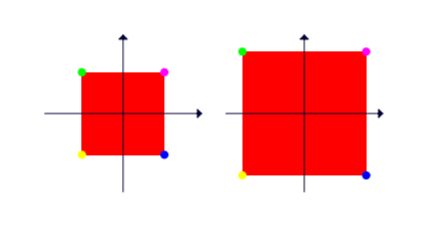
\includegraphics[width=10cm,keepaspectratio]{scale1}
% \end{frame}

% \begin{frame}{Outline}
  % \tableofcontents[hideallsubsections]
  % % You might wish to add the option [pausesections]
% \end{frame}

% Section and subsections will appear in the presentation overview
% and table of contents.

\section{극한} 

\subsection{극한의 정의} 


\begin{frame}[allowframebreaks]{무한의 직관적 이해}
가장 큰 자연수에 대해서 생각해 보자. 가장 큰 자연수는 몇인가? \\
애석하게도, 그러한 수는 존재하지 않는다. 어떤 자연수 N이 존재해서 그것이 가장 큰 자연수라고 한다면, N+1 역시 
\begin{itemize} 
\item 자연수이며
\item N보다 크므로
\end{itemize}
N은 가장 큰 자연수가 될 수 없다. 즉, 이에서 볼 수 있듯이 무한대를 어떠한 숫자로 생각하면 우리가 직관적으로 아는 무한대의 정의를 충족시킬 수 없다. 언제나 그 수에 1을 더해서 그 수보다 큰 수를 만들 수 있기 때문에, 무한대의 직관적인 정의인 어떠한 수보다 큰 수에 부합하지 않기 때문이다. 따라서 무한대는 숫자가 아니고, 다음을 만족하는 어떤 '것'으로 볼 수 있다. 

\begin{equation} 
\forall n, n < \inf
\end{equation}

보통 무한대는 계속 증가하는 '상태'로 해석하며, 이에 기반하여 앞으로의 논의를 진행할 것이다. 
\end{frame} 

\begin{frame}[allowframebreaks]{극한의 직관적 이해}

어떤 수열 $x_n$이 L에 '무한히' 접근한다고 하자. 이 때 무한히 접근한다는 것을 어떤 식으로 받아들여야 할까? 무한히 접근한다는 것은 여기서는 두 가지를 의미한다. 
\begin{itemize} 
\item $|x_n-L|$이 무한히 0에 접근한다. 
\item $x \neq a$ 이다. 
\end{itemize}

여기서 첫 번째 의미를 조금 더 살펴보자. 무한하게 0에 접근한다는 것은, 곧 다음과 같이 생각할 수 있다. 즉, 

\begin{equation} 
\forall \epsilon>0, \exists N, \forall n>N, |x_n-L| < \epsilon
\end{equation}

위 식을 도식화하면 아래와 같다. 

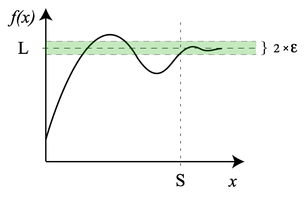
\includegraphics[width=10cm,keepaspectratio]{limit}

즉, 어떠한 $\epsilon$을 잡더라도, 충분한 시간이 지나면 (즉 충분히 n이 커지면) L과 $x_n$의 거리가 $\epsilon$이하로 유지된다면 우리는 $x_n$이 L에 무한히 접근한다고 생각할 것이다. 이제, 수열이 아니라 어떤 함수가 L에 접근하는 경우를 생각해 보자. 즉, x가 a로 무한히 접근할 때, f(x)가 L로 접근하는 것을 위와 같이 어떻게 나타낼지 생각해 보자. 먼저, 명제 형식으로 쓰면 다음과 같다. 

\begin{equation} 
(x \rightarrow a ) \rightarrow (f(x) \rightarrow L)
\end{equation}

즉, x가 a에 충분히 가까우면 f(x)와 L도 어느정도 가까워져야 할 것이다. 이 때, f(x)와 L이 가까워지는 정도에는 한계가 없어야 한다. 즉, 임의의 $\epsilon$만큼 가까워질 수 있어야 한다. 이 때, x와 a의 거리가 충분히 가까우면 되므로, 이 충분히 가까운 거리를 $\delta$라고 하자. 그러면 이를 정리해서 아래와 같이 쓸 수 있다. 

\begin{equation} 
\forall \epsilon \exists \delta 0<|x-a|<\delta \rightarrow |f(x)-L|< \epsilon
\end{equation}

\end{frame} 




\begin{frame}{$\epsilon-\delta$ 논법}
위 논의를 정리하면 다음과 같다. 

\begin{block}{극한} 
$lim_{x\rightarrow a} f(x) = L$ 은 $\forall \epsilon \exists \delta 0<|x-a|<\delta \rightarrow |f(x)-L| < \epsilon$
\end{block}

이 때, 좌극한과 우극한을 따로 다음과 같이 정의하며, 좌극한과 우극한이 같은 값일 때 극한이 존재한다고 한다. 

\begin{block}{좌/우극한} 
우극한은 $lim_{x\rightarrow a+} f(x) = L$ 은 $\forall \epsilon \exists \delta x-a<\delta \rightarrow |f(x)-L| < \epsilon$이라고 하며, x가 a보다 항상 큰 경우를 말한다. \\
좌극한은 $lim_{x\rightarrow a-} f(x) = L$ 은 $\forall \epsilon \exists \delta x-a<\delta \rightarrow |f(x)-L| < \epsilon$이라고 하며, x가 a보다 항상 작은 경우를 말한다. 
\end{block}
\end{frame} 

\begin{frame}{$\epsilon-\delta$ 논법을 이용한 증명}
위 논법을 이용하여 $f(x) = 2x+4$가 x가 0으로 갈 때, 4로 수렴하는 것을 증명해 보자. 
\begin{eqnarray} 
lim_{x \rightarrow 0} 2x+4 &\leftrightarrow& \forall \epsilon \exists \delta 0<|x|<\delta \rightarrow |2x+4-4|<\epsilon \\ 
& \leftrightarrow & \forall \epsilon \exists \delta 0<|x|<\delta \rightarrow 2|x|<\epsilon
\end{eqnarray}

따라서, $\delta = \frac{\epsilon}{2}$면 성립한다. 대개의 경우 , $\epsilon-\delta$ 논법을 이용한 극한의 증명은 적절한 $\delta(\epsilon)$을 찾는 것으로 귀결된다. 
\end{frame} 

\begin{frame}{$\epsilon-\delta$ 논법과 계산오차} 

$\epsilon-\delta$ 논법은 비단 수학적인 극한의 논의에서만 사용되는 것이 아니라, 계산오차의 예상에도 사용될 수 있다. 예컨대, 어떤 함수 f(x)를 수치적으로 계산한다고 하자. 이 때, 우리가 계산 결과인 f(x)의 계산오차를 줄이기 위해서는 입력인 x의 정확도를 높여야 한다. 하지만 얼마나 높여야 우리가 원하는 계산오차를 만족할 수 있을까? 

위 $\epsilon-\delta$ 논법에서 $\delta(\epsilon)$는 우리가 원하는 오차(혹은 input precision)에 대한 출력의 오차(precision)으로 생각할 수 있다. 즉, 우리가 원하는 계산결과의 정확도를 위해서 요구되는 입력값의 precision으로 생각할 수 있다. 예를 들어서, 위 예시에서 볼 수 있듯이 선형함수 ax+b를 출력오차 $\epsilon$ 내로 계산하기 위해서는 $a \epsilon$의 정확도로 x를 입력하면 된다. 

\end{frame}


\subsection{극한의 계산} 

\begin{frame}{극한의 연산}
함수 f, g가 $x \rightarrow a$일 때 각각 $\alpha, \beta$로 수렴한다면 다음이 성립한다. 
\begin{itemize} 
\item $lim(f+g) = \alpha + \beta$
\item $lim(fg) = \alpha \beta$
\item $lim(\frac{f}{g}) = \frac{\alpha}{\beta}$
\end{itemize}
여기서, 역은 성립하지 않는다. 
\end{frame} 



\subsection{함수의 극한}


\begin{frame}{연속함수}
다음을 만족하는 함수를 연속함수라고 한다. 

\begin{block}{연속함수} 
함수 f의 정의역의 모든 원소 a에 대해서, $lim_{x \rightarrow a} f(x) = f(a)$ 가 성립하면 f는 연속함수이다. 
\end{block}


\end{frame} 

\begin{frame}
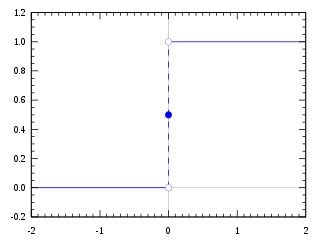
\includegraphics[width=10cm,keepaspectratio]{step}
\begin{itemize} 
\item 불연속함수 
\item Piecewise Continuous 함수 
\end{itemize}
\end{frame}

\section{미분} 

\subsection{함수의 미분} 

\begin{frame}{접선과 미분의 정의 }
곡선 y=f(x)위의 한 점 (a,f(a))에서의 접선 l은 다음과 같이 정의된다. 
\begin{block} {접선} 
접선 l은 두 점 P(a, f(a)), Q(b, f(b))로 이루어진 선분 PQ의 다음과 같은 극한이다. 

$lim_{b \rightarrow a} PQ$ 

\end{block}
정의에 따라서, 접선의 기울기는 다음과 같다. 

\begin{equation} 
lim_{x \rightarrow a} \frac{f(x)-f(a)}{x-a} = lim_{h \rightarrow 0} \frac{f(a+h)-f(a)}{h}
\end{equation}

위 식은 점 (a,f(a))에서 접선의 기울기를 뜻한다. 이제, 정의역 안 임의의 점에서 접선의 기울기를 생각해보면 접선의 기울기 역시 하나의 함수로 볼 수 있고, 이를 도함수, 혹은 함수의 미분이라고 한다. 함수의 x에 대한 미분은 $\frac{df}{dx} $나 $f^{\prime}$와 같이 쓴다. 

\end{frame} 

\begin{frame}{미분 연산 법칙과 그 증명}

미분가능한 함수 f,g에 대해서 다음이 성립한다. 
\begin{itemize} 
\item $\frac{d}{dx} cf = c \frac{df}{dx}$ 
\item $\frac{d}{dx} (f+g) = \frac{df}{dx} + \frac{dg}{dx}$ 
\item $\frac{d}{dx} (fg) = g\frac{df}{dx} + f\frac{dg}{dx}$ 
\item $\frac{d}{dx} \frac{f}{g} = \frac{f^{\prime}g-g^{\prime}f}{g^2}$
\item $\frac{d}{dx} f(g(x)) = \frac{d f(g(x))}{dg} \frac{dg}{dx}$ : Chain Rule 
\end{itemize}
\end{frame} 

% 증명 슬라이드 첨부 


\begin{frame}{다양한 함수의 미분}
\begin{itemize} 
\item 다항함수 : $\frac{d}{dx} a_ix^i = ia_ix^{i-1}$
\item 지수함수 : $\frac{d}{dx} e^x = e^x, \frac{d}{dx} a^x = a^x ln(a)$
\item 삼각함수 : $\frac{d}{dx} sin x = cos x , \frac{d}{dx} cos x = - sin x, \frac{d}{dx} tanx = \frac{1}{(cos x)^2} $
\item 로그함수 : $\frac{d}{dx} ln x = \frac{1}{x}, \frac{d}{dx} log_a x = \frac{1}{x ln a}$
\end{itemize}
\end{frame} 

% 증명 슬라이드 첨부 



\subsection{함수의 편미분} 

 

\begin{frame}{편미분}
다변수함수 $f(x_1, x_2, ..., x_n)$에 대해서, 변수 $x_i$로의 편미분은 다음과 같이 정의된다. 

\begin{equation} 
\frac{\partial f}{\partial x_i} = lim_{h \rightarrow 0} \frac{f(x_1, x_2, ..., x_i+h, ... x_n) - f(x_1, x_2, ..., x_i, ..., x_n)}{h}
\end{equation}

즉, 다변수함수에서 다른 변수들을 다 상수로 취급하고, 한 변수에 대한 미분만을 계산하는 것이 편미분이다. 따라서 계산 등은 상미분과 동일하다. 

\end{frame} 

\begin{frame}{Total Derivative} 
f(x(t), y(t))의 t에 대한 상미분 $\frac{df}{dt}$는 다음과 같다. 

\begin{equation}
\frac{df}{dt} = \frac{\partial f}{\partial x}\frac{dx}{dt} +  \frac{\partial f}{\partial y}\frac{dy}{dt}
\end{equation}
\end{frame}

\begin{frame}{Proof} 
미분의 정의에 따라서, 

\begin{equation} 
\frac{df}{dt} = lim_{h->0} \frac{f(x(t+h), y(t+h)) - f(x(t), y(t))}{h}
\end{equation}
이다. 우변을 다음과 같이 변형하자. 

\begin{eqnarray} 
&& \frac{f(x(t+h), y(t+h)) - f(x(t), y(t))}{h} \\
&=&  \frac{f(x(t+h), y(t+h)) - f(x(t+h), y(t)) + f(x(t+h), y(t)) - f(x(t), y(t))}{h} \\ 
&=& \frac{f(x(t+h), y(t+h)) - f(x(t+h), y(t))}{h} + \frac{f(x(t+h), y(t)) - f(x(t), y(t))}{h} \\
&=& \frac{f(x(t+h), y(t+h)) - f(x(t+h), y(t))}{y(t+h)-y(t)} \frac{y(t+h) - y(t)}{h} + \frac{f(x(t+h), y(t)) - f(x(t), y(t))}{x(t+h) - x(t)} \frac{x(t+h) - x(t)}{h}\\ 
&=& \frac{\partial f}{\partial y}\frac{dy}{dt} + \frac{\partial f}{\partial x}\frac{dx}{dt} 
\end{eqnarray}
\end{frame}

\begin{frame}{고차 편미분} 

다변수함수의 편미분은 상미분과는 다르게, 다른 변수들로 미분을 여러번 할 수 있다. 예컨대, 이변수함수 f(x,y)는 다음과 같은 두 가지 방법으로 두 번 편미분될 수 있다. 

\begin{eqnarray} 
\frac{\partial }{\partial x} \frac{\partial f}{\partial y} \\
\frac{\partial }{\partial y}\frac{\partial f}{\partial x}
\end{eqnarray}

이 두 식은, 두 식이 각각 연속이라면 같은 식이 된다. 이를 Clairaut's theorem on equality of mixed partials라고 한다. 


\end{frame}








\section{미분 연산자}

\subsection{선형 변환과 미분} 

\begin{frame}{연산자로써의 미분}

x에 대한 미분 $D_x = \frac{d}{dx}$는 함수에 대한 일종의 연산자로 볼 수 있다. 그런데, 미분 연산자는 
\begin{itemize} 
\item $D_x(cf(x)) = cD_x(f(x))$
\item $D_x(f(x) + g(x)) = D_x(f(x)) + D_x(g(x))$ 
\end{itemize}
로, 선형성을 가진다. 따라서 미분은 선형 변환이다. 이는 편미분도 똑같다. 
\end{frame} 

\subsection{벡터와 미분} 

\begin{frame}{벡터 함수}
벡터 함수 $\vec{f}$는 다음과 같이 정의된다. 

\begin{block}{벡터 함수} 
벡터 함수 $\vec{f}$는 함수 $f_1, f_2, ... , f_n$으로 만들어진 n-벡터이며, 다음과 같이 쓴다. 

$\vec{f} = (f_1, f_2, ..., f_n) $
\end{block}

벡터 함수의 연산은 일반적인 벡터와 함수의 연산을 따른다. 
\end{frame} 


\begin{frame}{벡터 함수의 미분과, 벡터로의 미분} 
벡터 함수의 x에 대한 편미분은 다음과 같이 정의된다. 

\begin{equation} 
\frac{\partial \vec{f}}{\partial x} = \left[ \begin{matrix} \frac{\partial f_1}{\partial x} \\ \frac{\partial f_2}{\partial x} \\ ... \\ \frac{\partial f_n}{\partial x} \end{matrix} \right]
\end{equation}

반대로, 벡터 $\vec{x} = (x_1, x_2, ..., x_n)$으로 스칼라함수 $f(x_1, x_2, ... , x_n)$을 미분하는 것은 다음과 같이 정의된다. 

\begin{equation} 
\frac{\partial f}{\partial \vec{x}} = \left[ \begin{matrix} \frac{\partial f}{\partial x_1} \\ \frac{\partial f}{\partial x_2} \\ ... \\ \frac{\partial f}{\partial x_n} \end{matrix} \right]
\end{equation}

\end{frame}

\begin{frame}{벡터와 벡터로의 미분}
\begin{equation} 
\frac{\partial \vec{y}}{\partial \vec{x}} = \left[ \begin{matrix} 
\frac{\partial y_1}{\partial x_1} & \frac{\partial y_1}{\partial x_2} & ... & \frac{\partial y_1}{\partial x_n} \\ 
\frac{\partial y_2}{\partial x_1} & \frac{\partial y_2}{\partial x_2} & ... & \frac{\partial y_2}{\partial x_n} \\ 
... & ... & ... & ... \\
\frac{\partial y_n}{\partial x_1} & \frac{\partial y_n}{\partial x_2} & ... & \frac{\partial y_n}{\partial x_n} \end{matrix} \right]
\end{equation}
\end{frame}

\begin{frame}{행렬의 미분과 행렬로의 미분} 
\begin{equation} 
\frac{\partial Y}{\partial x} = \left[ \begin{matrix} 
\frac{\partial y_{11}}{\partial x} & \frac{\partial y_{12}}{\partial x} & ... & \frac{\partial y_{1n}}{\partial x} \\ 
\frac{\partial y_{21}}{\partial x} & \frac{\partial y_{22}}{\partial x} & ... & \frac{\partial y_{2n}}{\partial x} \\ 
... & ... & ... & ... \\
\frac{\partial y_{n1}}{\partial x} & \frac{\partial y_{n2}}{\partial x} & ... & \frac{\partial y_{nn}}{\partial x} \end{matrix} \right]
\end{equation}

\begin{equation} 
\frac{\partial y}{\partial X} = \left[ \begin{matrix} 
\frac{\partial y}{\partial x_{11}} & \frac{\partial y}{\partial x_{21}} & ... & \frac{\partial y}{\partial x_{n1}} \\ 
\frac{\partial y}{\partial x_{12}} & \frac{\partial y}{\partial x_{22}} & ... & \frac{\partial y}{\partial x_{n2}} \\ 
... & ... & ... & ... \\
\frac{\partial y}{\partial x_{1n}} & \frac{\partial y}{\partial x_{2n}} & ... & \frac{\partial y}{\partial x_{nn}} \end{matrix} \right]
\end{equation}
\end{frame}




\begin{frame}[allowframebreaks]{$\nabla$ 연산자와 그 응용}
$\nabla$ 연산자는 델 연산자라고도 하며, 보통 3차원에서 정의된다. 본 수업에서도 3차원에서의 델 연산자만을 다룰 것이다. 
\begin{block}{$\nabla$ 연산자} 
$\nabla$는 다음의 3-벡터이다.

$\nabla = (\frac{\partial}{\partial x}, \frac{\partial}{\partial y}, \frac{\partial}{\partial z})$
\end{block}

델 연산자는 벡터이기 때문에 스칼라배와 내적이 가능하며, 또한 3차원에서는 외적도 가능하다. 각각이 벡터 함수의 연산에 대응된다. 
\begin{itemize} 
\item Gradient : 스칼라배 
\item Divergence : 내적 
\item Curl : 외적 
\end{itemize}
\end{frame} 

\begin{frame}[allowframebreaks]{Gradient}
스칼라 함수 f에 대해서, 그 함수의 gradient $\nabla f$는 다음과 같이 정의된다. 
\begin{block}{Gradient $\nabla f$} 
$\nabla f = (\frac{\partial f}{\partial x}, \frac{\partial f}{\partial y},\frac{\partial f}{\partial z}) = \frac{\partial f}{\partial x} \hat{x} + \frac{\partial f}{\partial y} \hat{y} + \frac{\partial f}{\partial z} \hat{z}$
\end{block}

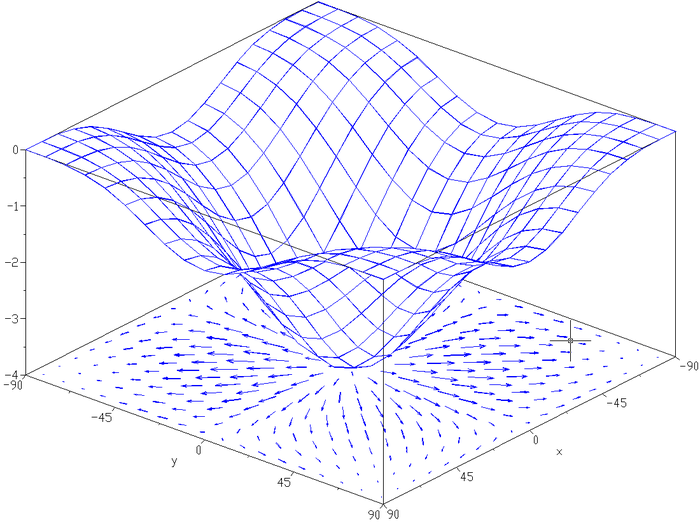
\includegraphics[width=10cm,keepaspectratio]{gradient}

함수의 그래디언트는 함수가 만드는 곡면에서의 기울기를 나타내는 벡터라고 할 수 있다. 그래디언트의 각 항을 살펴보면, $\hat{x}$항은 곧 곡면을 x충에 평행하게 자른 성분의 미분이라고 볼 수 있다. 
\end{frame} 



% \begin{frame}{Divergence}
% \begin{itemize} 
% \item 
% \end{itemize}
% \end{frame} 

% \begin{frame}{Curl}
% \begin{itemize} 
% \item 
% \end{itemize}
% \end{frame} 

% \begin{frame}{여러 정리와 그 증명}
% \begin{itemize} 
% \item 
% \end{itemize}
% \end{frame} 

\section{미분의 응용}

\subsection{미분과 극값} 

\begin{frame}{극값}
극값은 극소점과 극대점을 통틀어 말하며, 이는 local minimum과 local maximum을 통칭한다. local minimum과 local maximum은 각각 다음과 같이 정의된다. 

\begin{block}{Local Minimum/Maximum }
함수 f에 대해서, 다음의 집합의 원소를 극점이라 한다. 
$\{x* \in X| \exists d \forall x \in |x-x*|<d, f(x*) > x ````or ````f(x*) < x\}$
\end{block}

1) 극값에서는 도함수가 0이다. 하지만, 그 역은 성립하지 않는다. 

\end{frame} 

\begin{frame}{Proof of 1)}
함수 f가 x=a에서 극댓값을 가진다고 하자. 이 때, 도함수의 1)좌극한과 2)우극한의 부호가 다르기 때문에, 수렴하기 위해서는 도함수가 0이여야 함을 이용하여 보일 것이다. 극소값일 경우도 대칭적으로 증명하면 된다. 

1) 극댓값의 정의에 따라서 어떤 $\delta$가 존재해서, $(a-\delta, a+\delta)$ 구간 안의 모든 원소 x에 대해서 f(x)<f(a)이다. 이제, $(a-\delta, a)$ 구간에서 함수의 도함수를 생각하자. 이 구간의 원소인 x에 대해서 항상 x-a<0이며, 극댓값의 정의에 따라서 f(x)-f(a)>0이다. 따라서 $\frac{f(x)-f(a)}{x-a}\leq 0$ 이다. 

2) 1)과 같이 $\delta$를 잡자. 이 때 $(a, a+\delta)$의 값을 잡자. 위 논의와 비슷하게, 결국 $\frac{f(x)-f(a)}{x-a}\geq 0$가 된다. 

즉, 좌극한은 0 이하이고, 우극한은 0 이상이다. 좌극한과 우극한이 같아야 수렴하므로, 미분가능한 함수라면 극값에서 도함수가 0이 되어야만 한다. 

역의 반례는 $y=x^3$에서 x=0이다.  
\end{frame} 

% 증명 슬라이드 첨부 

\begin{frame}{함수에서 극값의 탐색}
함수 f에 대해서, 다음과 같이 탐색한다. 
\begin{itemize} 
\item 일변수함수의 경우 : $\frac{df}{dx}=0$의 해를 구하고, 극값의 조건을 만족하는지 판별한다. 
\item 다변수함수의 경우 : 함수 $f=f(x_1, x_2, ..., x_n)$에 대하여, $\frac{\partial f}{\partial x_i}=0$의 연립방정식을 만족하는 해를 구하고, 극값의 조건을 만족하는지 판별한다. 
\end{itemize}
\end{frame}


\begin{frame}[allowframebreaks]{다변수함수에서 제약조건이 주어졌을 때 극값의 탐색} 


어떤 이변수함수 f(x,y)의 극값을 g(x,y)라는 조건이 주어졌을 때 구하는 문제를 생각해 보자. 예를 들어서, $f = x^2+y^2,`` g = x^2+xy+y^2-1$이라고 하자. 이 때 f의 최댓값을 구하는 문제를 생각해 보자.

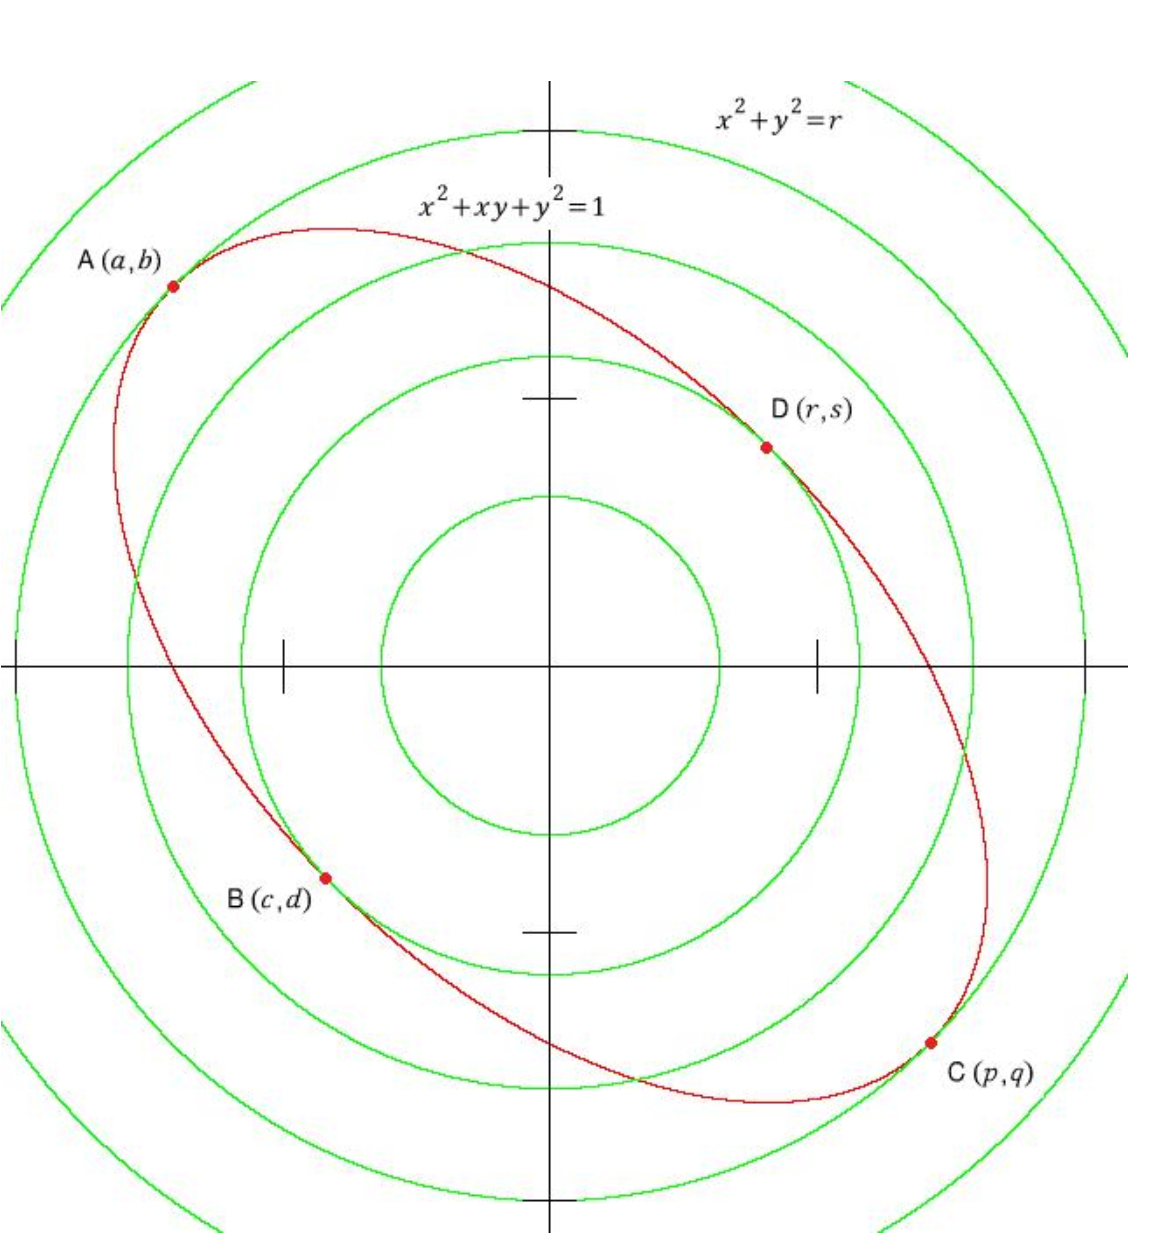
\includegraphics[height=5cm,keepaspectratio]{lag}

 위 그림에서 볼 수 있듯이, f는 원점을 중심으로 하는 원이다. 이 원들 중에서 주어진 곡선 g와 공통접선을 가지는 점이 극값이 됨을 관찰할 수 있다. 이에 착안하여, 본 문제는 다음과 같이 풀 수 있다. 즉, 점 A(a,b)에서 두 곡선 $f=x^2+y^2-r^2, `` g = x^2+xy+y^2-1$은 $\nabla f = \alpha \nabla g$를 만족한다. 

그렇다면, 우리는 다음과 같은 생각을 할 수 있다. 즉, 극값을 가지는 점 $(x_0, y_0)$에 대해서, $\nabla f (x_0, y_0) = \lambda \nabla g(x_0, y_0)$가 성립한다. 즉, 

\begin{eqnarray} 
\nabla f(x,y) &=& \lambda \nabla g(x,y) \\
g(x,y) &=& 0
\end{eqnarray}

의 연립방정식을 풀면 극값을 구할 수 있을 것이다. 조금 더 엄밀하게는, 이러한 $\lambda$가 언제나 존재한다. 즉, 

\begin{block}{라그랑주 승수법} 
함수 f(x,y)가 g(x,y) = 0 위의 점 $(x_0, y_0)$에서 극값을 가질 때, 적당한 실수 $\lambda$에 대해서 다음이 성립한다. 

$\nabla f(x_0, y_0) = \lambda \nabla g(x_0, y_0)$ 

이 때, $\nabla g(x_0, y_0) \neq 0$이다. 
\end{block}
이러한 방법을 라그랑주 승수법이라고 하며, $\lambda$를 라그랑주 승수라고 한다. 

\end{frame}

\begin{frame}[allowframebreaks]{Proof} 
곡선 g(x,y) = 0 위의 한 점을 다음의 벡터함수 $x(t), y(t)$로 생각하자. 이 때, g(x,y) = 0 곡선 위의 f는 다음과 같이 쓸 수 있다. 

\begin{equation} 
z = f(x(t), y(t))
\end{equation}

라고 할 수 있다. 이 때, f가 극값을 $(x_0, y_0)$에서 가진다고 하고, 
\begin{eqnarray}
x_0 = x(t_0) \\ 
y_0 = y(t_0)
\end{eqnarray}
라고 하자.  그러면 $\frac{dz}{dt}(t=t_0) = 0$이므로, 다음이 성립한다. 

\begin{eqnarray} 
\frac{dz}{dt} &=& \frac{\partial f}{\partial x}\frac{dx}{dt} + \frac{\partial f}{\partial y}\frac{dy}{dt} \\ 
&=& (\frac{\partial f}{\partial x}, \frac{\partial f}{\partial y}) \bullet (\frac{dx}{dt}, \frac{dy}{dt}) \\
&=& \nabla f \bullet (\frac{dx}{dt}, \frac{dy}{dt})
\end{eqnarray}

즉, $\nabla f$와 $(\frac{dx}{dt}, \frac{dy}{dt})$는 수직하다. 또한, 접선과 gradient 역시 수직하므로 $\nabla g$와 $(\frac{dx}{dt}, \frac{dy}{dt})$ 역시 수직하다. 따라서 $\nabla f$와 $\nabla g$ 는 평행하다. 
\end{frame}

\begin{frame}{Intermediate Value Theorem} 
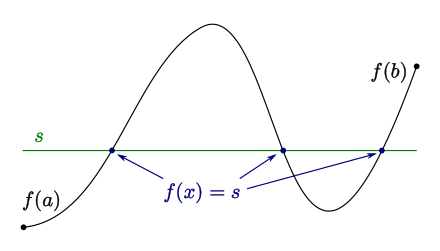
\includegraphics[height=5cm,keepaspectratio]{ivp}
\begin{block}{Intermediate Value Theorem} 
연속함수 f에 대해서, 정의역 내 구간 [a,b]에 대하여 f(a)<s<f(b)인 s에 대하여, f(c)=u인 c가 (a,b)에 존재한다. 
\end{block}

이는 실수의 완비성을 이용하여 증명할 수 있으나, 본 수업의 scope를 벗어나므로 여기서는 생략하고 IVP를 받아들이기로 한다. 

\end{frame}

\begin{frame}{Mean Value Theorem}
\begin{block}{Mean Value Theorem} 
함수 f가 연속이고 미분 가능하면, 어떤 정의역 내 구간 (a,b)에 대해서 

$\frac{df}{dx}(x=c) = \frac{f(b)-f(a)}{b-a}$

인 c가 (a,b) 내에 존재한다. 
\end{block}

이의 특이한 케이스로, 롤의 정리도 있다. 

\begin{block}{Rolle's Theorem}
f(a) = f(b)라면, $f^{\prime}(c)=0$인 c가 (a,b) 내에 있다. 
\end{block}
\end{frame}
\begin{frame}{Proof of MVT} 
먼저, 롤의 정리를 증명하자. (a,b) 내에 만약 극값이 있다면, 극값은 $f^{\prime} = 0$을 만족하므로 성립한다. 만약 없다면, f(x)는 (a,b) 내에서 상수함수이므로 모든 구간에서 $f^{\prime} = 0$이므로 성립한다. 

MVT는 $g(x) = f(x) + \frac{f(b)-f(a)}{b-a}(x-a)+f(a)$ 로 변형하고 롤의 정리를 대입하면 바로 증명된다. 
\end{frame}

\begin{frame}[allowframebreaks]{테일러 급수} 
\begin{block}{테일러 정리} 
만약 f가 (n+1)번 미분가능한 함수라면, 정의역 내의 구간 (a,b)에 대해서 다음을 만족하는 c가 존재한다. 

$f(b) = f(a) +  \sum_{i=1}^n \frac{f^{(i)}(a)}{i!} +\frac{ f^{(n+1)}(c)}{(n+1)!} (b-a)^{(n+1)}$
\end{block}

여기서 테일러급수는 

\begin{equation} 
f(x) = f(a) + \sum_{i=1}^n \frac{f^{(i)}(a)}{i!} + R_n(x) = T_n(x) + R_n(x)
\end{equation}

이며, remainder function $R_n$은 

\begin{equation} 
R_n(x) = \frac{f^{(n+1)}(c(x))}{(n+1)!}(x-a)^{n+1}
\end{equation}
이다. 

만약 $|f^{(n+1)}(x) \leq M|$으로 bound된다면, $R_n(x)$ 또한 bound되므로 모든 n에 대해서 $|f^{(n+1)}(x) \leq M|$가 성립한다면 테일러급수 $T_n(x)$는 f(x)로 수렴하게 된다. 
\end{frame}

\begin{frame}{다음시간 실습 및 숙제 : symbolic 미분의 구현} 

\begin{itemize} 
\item tokenizer/parser에 func token 추가 
\item 상미분, 편미분 구현
\item 벡터-스칼라, 스칼라-벡터, 벡터-벡터, 행렬-스칼라, 스칼라-행렬간의 미분 구현 
\item $\nabla$의 구현 
\item  주어진 함수의 n차 테일러 전개 구현 
\end{itemize}

숙제이기는 하지만 꼭 해 볼 필요는 없습니다. 할 때 git merge confilct를 피하기 위해서 practices/ 폴더를 만들어서, skeleton 폴더의 모든 것을 복사하고 해 보시길 권장드립니다. practices/ 폴더는 gitignore에 추가되어 있으므로 에러가 나지 않으며, 연습할 때 편리할 것입니다. 
\end{frame}


\begin{frame}{tokenizer/parser에 token 추가} 

다음과 같은 순서로 하기를 권장함. 
\begin{itemize} 
\item 미리 정해진 함수와 도함수의 dict를 만듬. key는 str, value는 2-tuple로 파이썬 함수와 도함수를 담고 있는 PyFormula 인스턴스로 구성한다. 
\item tokenizer를 받아서, var들의 모임들 중 앞 과정에서 지정한 함수들에 해당하는 알파벳이 들어오는지를 판별, func로 함수 토큰을 생성. 
\item parser에서 func 토큰 핸들링하는 부분을 unary와 비슷하게 만들되, (와 ,로 argument를 구분할 수 있도록 한다. 
\end{itemize}

func 토큰에는 sin, cos, ln, e, pi를 꼭 포함하여야 한다. e와 pi는 상수함수이다. 
\end{frame}


\begin{frame}{Symbolic 미분의 구현} 
미분은 PyFormula 인스턴스를 입력받아, PyFormula 인스턴스를 리턴하는 PyCalculus.py/differentiate 함수를 구현하는 것으로 한다. differentiate 함수는 다음 입력들을 받는다. 
\begin{itemize} 
\item formula : 미분할 PyInstanace 객체 
\item variable : 미분할 변수명 
\item constant\_variables : 변수이되, 상수 취급할 변수. 이외의 변수들은 모두 변수로 취급되어, 상미분시 도함수를 남겨야 한다. 예컨대, x로 미분할 경우 y가 변수라면 $\frac{dy}{dx}$가 리턴되어야 한다. 
\item is\_partial : 편미분일 경우 True
\item is\_symbolic : symbolic 미분일 경우 True. 본 실습에서는 True만들 사용한다. 
\end{itemize}
\end{frame}

\begin{frame}{Symbolic 미분의 구현 : 상미분}

다음과 같은 순서로 구현하기를 권장한다. 

\begin{itemize} 
\item if is\_symbolic 안에서 모든 것을 구현한다. 
\item formula의 형태에 따라서 재귀적으로 미분을 구현한다. formula 트리의 루트의 datum에 따라 다음과 같이 구현한다. 
\begin{itemize} 
\item operation인 경우 : 미분의 연산법칙에 따라 구현한다. 
\item func인 경우 : func가 정의된 dict로 가서, 도함수를 이용하여 구현한다. 이 때 chain rule을 사용한다. 다변수함수의 경우, 전미분을 이용하여야 함에 유의하자. 
\item var인 경우 : 미분하려는 변수이면 1, 상수 변수이면 0, 그렇지 않으면 미분하려는 변수에 대한 도함수를 리턴한다. 
\item num인 경우 : 0을 리턴한다. 
\end{itemize}
\end{itemize}

\end{frame}

\begin{frame}{Symbolic 미분의 구현 : 편미분}

위와 다 같으나, 두 가지의 차이가 있다. 

\begin{itemize} 
\item var인 경우 : 미분하려는 변수의 경우 1, 나머지의 경우 0. 
\item func인 경우 : 전미분이 아니라 편미분을 사용함에 유의. 
\end{itemize}
\end{frame}

% \begin{frame}{벡터/스칼라의 미분} 
% PyVector의 
% \end{frame}

% \begin{frame}{$\nabla$의 구현}

% \end{frame}

\begin{frame}{테일러급수의 구현} 

PyCalculs.py/taylor\_expansion 함수를 구현하라. input은 formula와 a, n 두 개이며, n번째 테일러급수의 항까지 리턴하는 PyFormula의 리스트를 만들면 된다. a는 실수로, a 근방에서 전개된 테일러급수를 구하면 된다. 

\end{frame}



% \begin{frame}[allowframebreaks]{다음시간 실습 및 숙제 : Gradient Descent의 구현}
% Gradient Descent는 다변수함수의 극값을 수치적으로 찾아내는 방법 중 하나이다. 일반적으로 시작점 $\vec{a}_0$에서 

% \begin{equation} 
% \vec{a}_{n+1} = \vec{a}_n - \gamma_n \nabla F(\vec{a}_n)
% \end{equation}

% 으로 수열을 진행, $\vec{a}_n$이 local minimum으로 수렴할 것을 \textbf{희망}한다. 여기서 희망한다는 것은 항상 그렇게 된다는 보장이 없다는 뜻이다. 
% \end{frame}



    

% \section{미분 방정식} 

% \subsection{1차 미분 방정식} 

% \subsection{n차 미분 방정식} 

% \subsection{선형 미분 방정식} 

\end{document}


